\section{Algoritmo de Holt Winters}
El método Holt-Winters es un método de pronóstico de triple exponente suavizante y tiene la ventaja de ser fácil de adaptarse a medida que nueva información real está disponible. El método Holt- Winters es una extensión del método Holt que considera solo dos exponentes suavizantes. Holt-Winters considera nivel, tendencia y estacional de una determinada serie de tiempos. 
\\ \par
El método de Holt-Winters es básicamente un procedimiento de suavizamiento exponencial. Este tipo de procedimientos facilitan los cálculos y reducen los requerimientos de almacenamiento en las bases de datos, lo cual cobra importancia cuando se están prediciendo muchas series de tiempo [1].
\\ \par

Existen tres fases de trabajo, con tres conjuntos de datos diferentes. 
\begin{itemize}
\item Un primer grupo de datos es para inicializar
el modelo, esto es determinar los indicadores de nivel, tendencia y estacionalidad. 
\item Un segundo conjunto de datos es necesario para probar o calibrar los índices de suavización Alfa, Beta y Gamma.
\item Un tercer grupo de datos para pronosticar y evaluar el funcionamiento del modelo propuesto.
\end{itemize}
Ejecutar todas las fases en un solo grupo de datos puede conducir a tratar de encajar en exceso el modelo a los datos disponibles [2].
\\ \par
Una vez que ya se ha explicado a grandes rasgos el funcionamiento del algoritmo de Holt Winters, se explicará paso a paso el procedimiento de la aplicación de dicho algoritmo.
\\ \par 
Primero se añadió el agente desde el cual se obtuvieron los datos en tiempo real tal y como se muestra en la figura \ref{image:agente}. 
\FloatBarrier
\begin{figure}[htbp!]
		\centering
			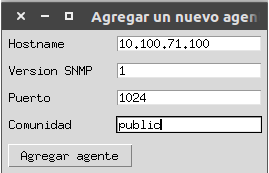
\includegraphics[width=.45 \textwidth]{images/agente}
		\caption{Nuevo agente añadido.}
		\label{image:agente}
\end{figure}
\FloatBarrier

Y de los agentes añadidos, se mostró la información en la pantalla principal como se observa en la figura \ref{image:agentes}. En esta imagen no se observa que el agente se encuentre activo debido a que su ejecución se realizó directamente en el laboratorio, sin embargo, en la figura \ref{image:agentes2} se muestran los datos del host 10.100.71.100 cuando este se encontraba activo.
\FloatBarrier
\begin{figure}[htbp!]
		\centering
			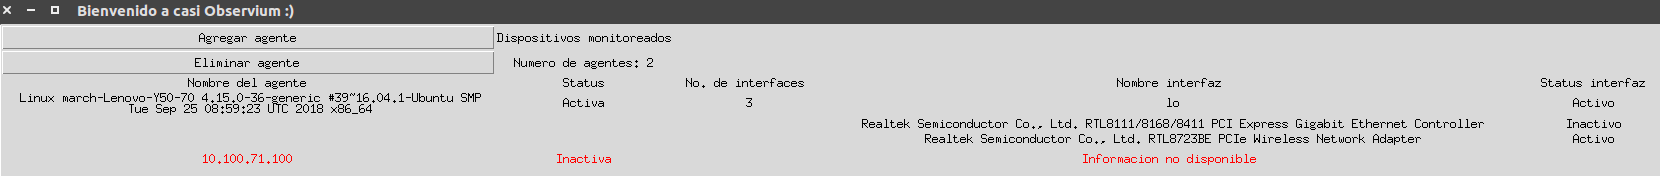
\includegraphics[width=1.1 \textwidth]{images/agentes}
		\caption{Pantalla principal de agentes.}
		\label{image:agentes}
\end{figure}
\FloatBarrier
\FloatBarrier
\begin{figure}[htbp!]
		\centering
			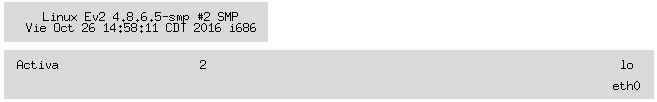
\includegraphics[width=1 \textwidth]{images/datos1}
		\caption{Información del agente activo.}
		\label{image:agentes2}
\end{figure}
\FloatBarrier

Una vez que el agente fue añadido, en los botones que se encuentran a lado derecho se pulsó sobre el botón con la leyenda \textbf{Graficos}, mismo que desplegaba una ventana con las opciones siguientes (figura \ref{image:graficos}):
\FloatBarrier
\begin{figure}[htbp!]
		\centering
			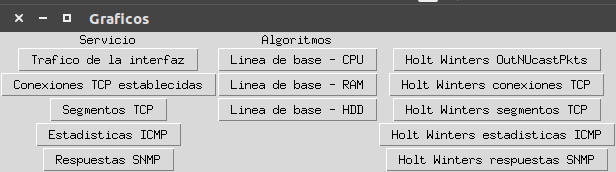
\includegraphics[width=.8 \textwidth]{images/graficos}
		\caption{Ventana de gráficos disponibles.}
		\label{image:graficos}
\end{figure}
\FloatBarrier
Al ser el equipo 10, nos fue asignado el monitoreo del OID de los \textbf{OutNUCastPkts}, por tal motivo se presionó sobre el primer botón y al realizar dicha acción se comenzó el monitoreo de los paquetes mostrando una gráfica similar a la de la figura \ref{image:grafica1}.
\FloatBarrier
\begin{figure}[htbp!]
		\centering
			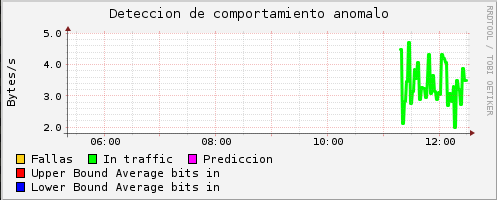
\includegraphics[width=.7 \textwidth]{images/grafica1}
		\caption{Gráfica de OutNUCastPkts.}
		\label{image:grafica1}
\end{figure}
\FloatBarrier
Misma que posteriormente y conforme fueron surgiendo los distintos fallos se mostró como las gráficas de a continuación:
\FloatBarrier
\begin{figure}[htbp!]
		\centering
			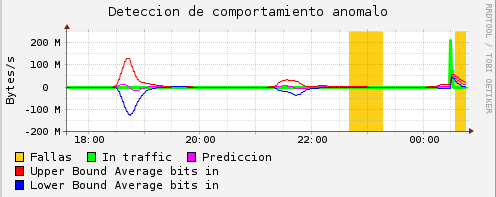
\includegraphics[width=.7 \textwidth]{images/grafica2}
		\caption{Gráfica de OutNUCastPkts.}
		\label{image:grafica2}
\end{figure}
\FloatBarrier

Sin embargo, también se realizaron mediciones con otros paquetes tal y como la gráfica de la figura \ref{image:grafica3} en la cual se plasman los datos obtenidos con el OID de \textbf{InOctets}.
\FloatBarrier
\begin{figure}[htbp!]
		\centering
			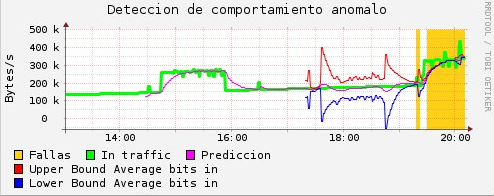
\includegraphics[width=.7 \textwidth]{images/grafica3}
		\caption{Gráfica de InOctets.}
		\label{image:grafica3}
\end{figure}
\FloatBarrier

Y como se observa en las gráficas mostradas anteriormente, una línea amarilla vertical marca las secciones en las cuales se ha sobrepasado el límite inferior o superior. Cuando dicho error sucede, se envían dos correos electrónicos al administrador indicando tanto el inicio del error como el final del mismo y adjuntando en dicho correo las gráficas como se puede observar en las figuras a continuación:
\\ \par
Respecto a los datos de entrada de OutNUCastPkts entre los correos recibidos se observan los de las figuras \ref{image:inicio} y \ref{image:fin}.
\FloatBarrier
\begin{figure}[htbp!]
		\centering
			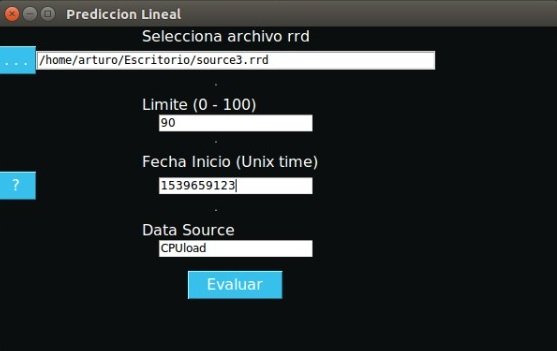
\includegraphics[width=.5 \textwidth]{images/inicio}
		\caption{Correo de inicio del error.}
		\label{image:inicio}
\end{figure}
\FloatBarrier
\FloatBarrier
\begin{figure}[htbp!]
		\centering
			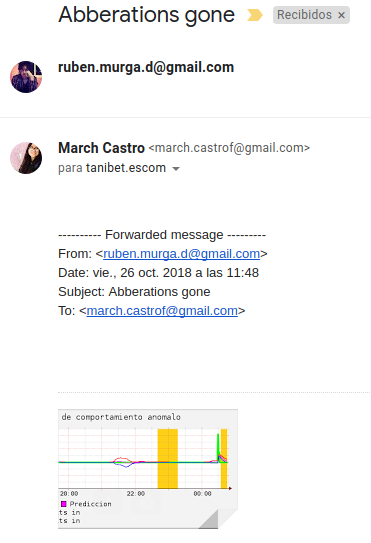
\includegraphics[width=.4 \textwidth]{images/fin}
		\caption{Correo de fin del error.}
		\label{image:fin}
\end{figure}
\FloatBarrier
Por otro lado, respecto a los datos de entrada de InOctets entre los correos recibidos se observan los de las figuras \ref{image:inicio1} y \ref{image:fin1}.
\FloatBarrier
\begin{figure}[htbp!]
		\centering
			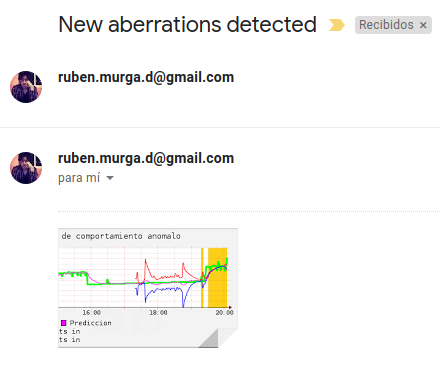
\includegraphics[width=.5 \textwidth]{images/inicio1}
		\caption{Correo de inicio del error.}
		\label{image:inicio1}
\end{figure}
\FloatBarrier
\FloatBarrier
\begin{figure}[htbp!]
		\centering
			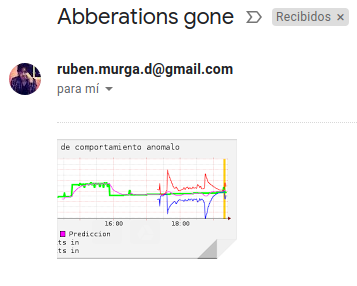
\includegraphics[width=.45 \textwidth]{images/fin1}
		\caption{Correo de fin del error.}
		\label{image:fin1}
\end{figure}
\FloatBarrier

\subsection{Explicación de código}
En esta sección se explicarán las partes del código más importante. En el método \textbf{actualizarHW} mostrado en la figura \ref{image:codigo4}, lo primero que se realiza es al momento de obtener por parámetros los datos del host al cual se desea gráficar, se verifica si existe ya un archivo .rrd en el cual ya se almacenen los datos, en caso contrario se manda a llamar al método \textbf{crearHW}.
\FloatBarrier
\begin{figure}[htbp!]
		\centering
			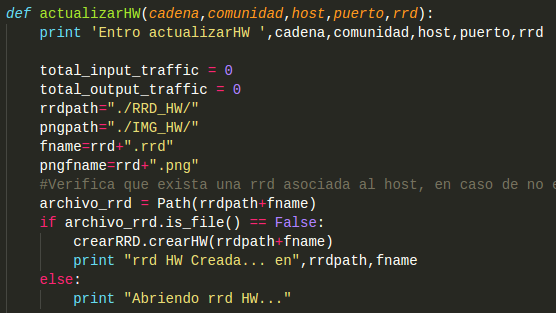
\includegraphics[width=.7 \textwidth]{images/codigo4}
		\caption{Método actualizarHW.}
		\label{image:codigo4}
\end{figure}
\FloatBarrier


El método \textbf{crearHW}, mostrado en la figura \ref{image:codigo1} se encarga de crear el archivo .rrd en el cual se almacenarán los datos indicados que en este caso se refieren a los datos de entrada de OutNUCastPkts.
\FloatBarrier
\begin{figure}[htbp!]
		\centering
			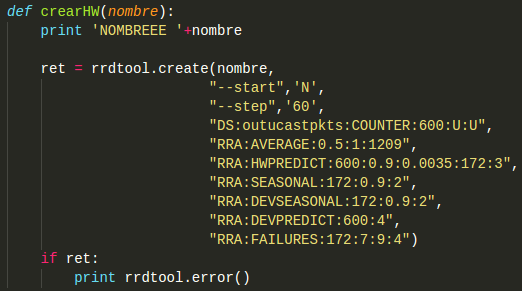
\includegraphics[width=.7 \textwidth]{images/codigo1}
		\caption{Método crearHW.}
		\label{image:codigo1}
\end{figure}
\FloatBarrier

\newpage
Una vez que se ha creado la base rrd, volvemos al códgo completo del método \textbf{actualizarHW} mostrado en la figura \ref{image:codigo3}, en el cual se obtienen los datos de entrada que se almacenan en la variable \textit{total\_input\_traffic}, utilizando el protocolo SNMP al  cual se indica el OID, hostname, puerto y nombre de la comunidad y con dichos datos obtenidos, se actualiza el archivo .rrd y con el comando .dump, se envian esos datos a un archivo .xml que es legible para el usuario.
\FloatBarrier
\begin{figure}[htbp!]
		\centering
			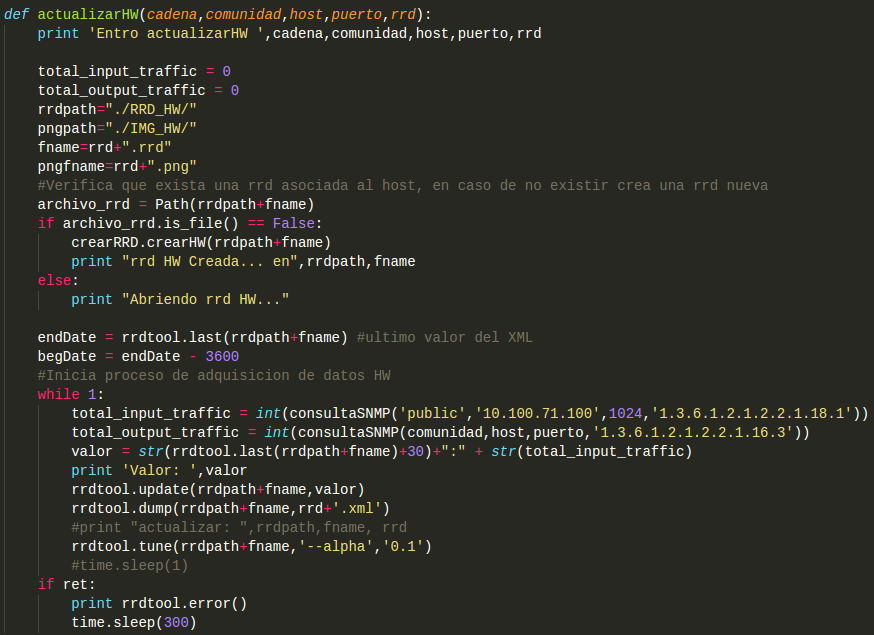
\includegraphics[width=1 \textwidth]{images/codigo3}
		\caption{Método actualizarHW.}
		\label{image:codigo3}
\end{figure}
\FloatBarrier

Posteriormente, la figura \ref{image:codigo2} muestra el código utilizado para realizar la graficación de los valores que se estan leyendo desde el archivo .rrd. En este método se indican que valores se desean gráficar, los colores y lo que significará cada una de las etiquetas mostradas en la parte inferior de la gráfica.
\FloatBarrier
\begin{figure}[htbp!]
		\centering
			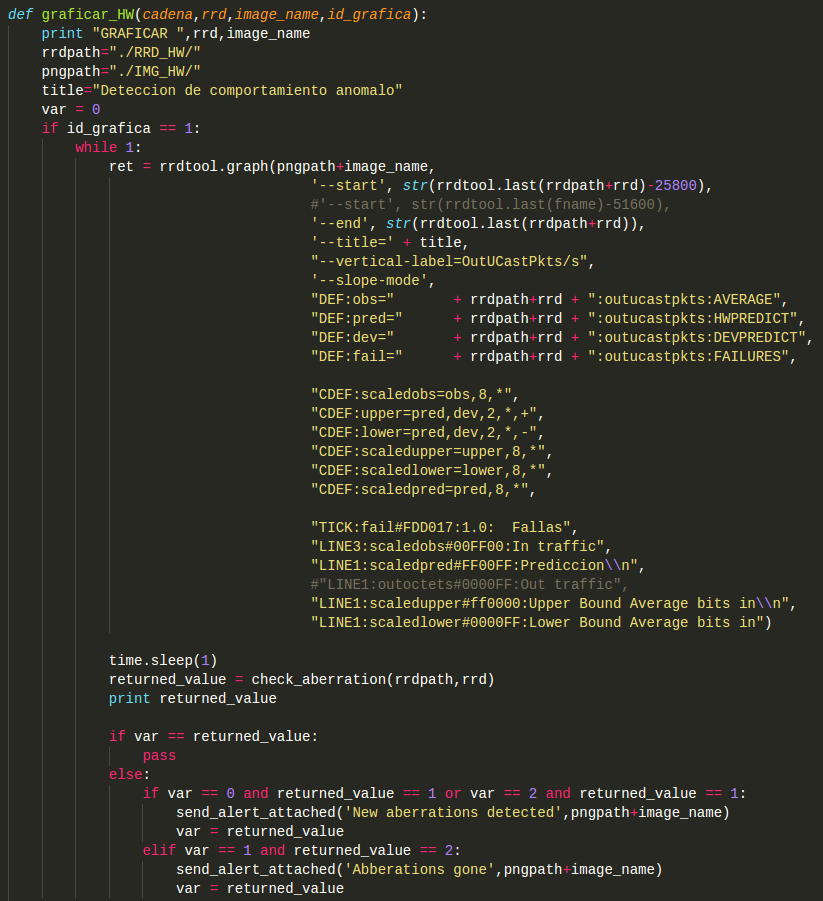
\includegraphics[width=1 \textwidth]{images/codigo2}
		\caption{Método graficar\_HW.}
		\label{image:codigo2}
\end{figure}
\FloatBarrier
Por último, las figuras \ref{image:codigo5} y \ref{image:codigo6} muestran los métodos encargados de revisar los datos en búsqueda de un cambio de valores en los fallos y en caso de encontrarlo se realiza el envío del correo electrónico.\\
El método check\_aberration se encarga de verificar los datos que se generan en los fallos mismos que solo toman un valor de 0 o 1, en caso de que el valor haya cambiado de 0 a 1, significa que un fallo ha comenzado, si el valor cambia de 1 a 0, significará que el fallo ha finalizado.
\FloatBarrier
\begin{figure}[htbp!]
		\centering
			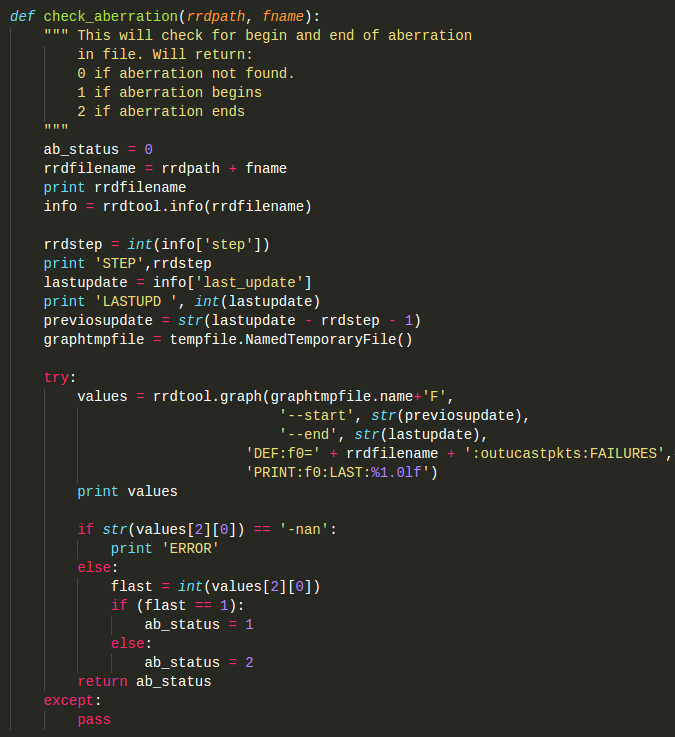
\includegraphics[width=.75 \textwidth]{images/codigo5}
		\caption{Método check\_aberration.}
		\label{image:codigo5}
\end{figure}
\FloatBarrier
\newpage
Por otro lado, el método se encarga de enviar el correo correspondiente con el titular necesario para indicar si el fallo comenzó o finalizó y anexando la imagen de la gráfica en el punto en el cual comenzó o termino dicho fallo.
\FloatBarrier
\begin{figure}[htbp!]
		\centering
			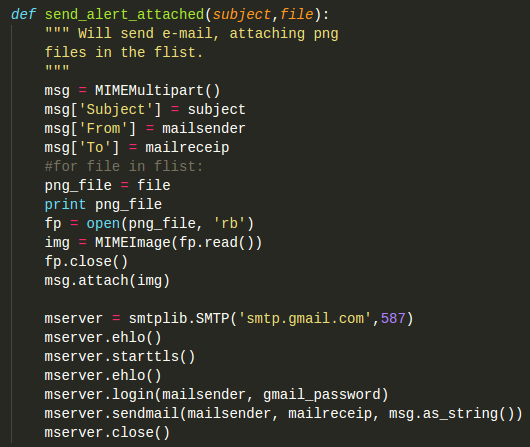
\includegraphics[width=.7 \textwidth]{images/codigo6}
		\caption{Método send\_alert\_attached.}
		\label{image:codigo6}
\end{figure}
\FloatBarrier
